\documentclass[12pt, letterpaper]{article}
\usepackage[margin=1in]{geometry}
\usepackage[utf8]{inputenc}
\usepackage{amsmath}
\usepackage{listings}
\usepackage{graphicx} 
\usepackage{fancyhdr}
\usepackage{booktabs} % For formal tables
\usepackage{float}
\usepackage{hyperref}
\usepackage{indentfirst}
\usepackage{multicol}
\usepackage{bookmark}
\usepackage[T1]{fontenc}
\usepackage{inconsolata}
\usepackage{listings}
\usepackage{color}
\usepackage{xcolor}

\renewcommand{\baselinestretch}{0.9}
\renewcommand{\rmdefault}{ptm}

\pagestyle{fancy}
\fancyhf{}
\setlength{\headheight}{15pt}
\rhead{Nicholas Quandt}
\lhead{McMaster Add-In for Autodesk Inventor}
\rfoot{Page \thepage}


\definecolor{bluekeywords}{rgb}{0.13,0.13,1}
\definecolor{greencomments}{rgb}{0,0.5,0}
\definecolor{redstrings}{rgb}{0.9,0,0}
\lstdefinestyle{sharpc}{language=[Sharp]C,
showspaces=false,
showtabs=false,
breaklines=true,
showstringspaces=false,
breakatwhitespace=true,
escapeinside={(*@}{@*)},
commentstyle=\color{greencomments},
keywordstyle=\color{bluekeywords},
stringstyle=\color{redstrings},
basicstyle=\ttfamily,
frame=lr,
rulecolor=\color{blue!80!black}
}

\begin{document}
\begin{titlepage}
   \begin{flushright}
       \vspace*{5cm}
 
       {\Huge \textbf{Software Requirements Specification}}
 
       \vspace{0.5cm}
        McMaster-Carr Add-In for Autodesk Inventor (MAFI)\\
        Version 1.0.2 $\bullet$ October 28 2019
 
       \vspace{1.5cm}
 
       \textbf{Nicholas Quandt}
       \\
       nicholas.quandt@marquette.edu
       \vfill
       Marquette University Masters Student of\\
       Computational Mathematical and Statistical Sciences\\
       \vspace{1cm}
 
   \end{flushright}
\end{titlepage}


\tableofcontents
\newpage

\section{Introduction}
\subsection{Purpose}
The purpose of this document is to detail the requirements of the "McMaster-Carr Add-In for Autodesk Inventor". It will describe the purpose, features, and future goals of the software. Further, it will examine the interface of both it and its parent application to the extent that a user who is familiar with the parent application can understand the new software implementation. This document will also list any constraints present, such as required operation system. The overall intent of this document is to allow a user to determine if this product would be of use.
\subsection{Document Conventions and Definitions}
This document was created based on the IEEE guide to system requirement specifications \cite{SRSTemplate}. The following describes all naming conventions used throughout the document:
\begin{itemize}
    \item MAFI: The McMaster-Carr Add-In for (Autodesk) Inventor software.
    \item Inventor: The computer application "Autodesk Inventor 2019" developed by Autodesk, Inc.\cite{Inventor}.
    \item McMaster: The online catalog available at www.mcmaster.com\cite{McMaster}.
    \item API: Application programming interface.
    \item 3D model: A three dimensional representation of a physical object, as shown within a computer program such as Inventor.
    \item Add-in: A software that relies on a parent application in order to execute, typically embedded within the parent application, i.e. non-standalone.
    \item IProperties: A set of attributes embedded within each Inventor file such as part number, description and physical material.
    \item Button: A user interface element that executes a process of an application from a mouse click.
    \item .NET: A software framework developed by Microsoft that includes a large class library and provides language interoperability across several programming languages\cite{NET}.
    \item CefSharp: A fast, fully embedded web browser for .NET applications\cite{CEFSharp}.
\end{itemize}
\subsection{Intended User}
\begin{itemize}
    \item Users of the program Autodesk Inventor 2019.
    \item Autodesk company employees who may want to further implement this software.
    \item Other parametric modelling application users who may want to implement similar software in another primary application.
\end{itemize}
\subsection{Product Scope}
MAFI will be an application add-in built for Inventor as a method for more efficiently connecting to, and retrieving models from, the McMaster database of 3D models that are used by mechanical designers. It will allow for a, direct, in-program access to the online catalog. Along with, "fast" conversion of the database file-type into something usable by an Inventor user. This is a software that should speed up design projects for engineers who use 3D models available from McMaster, within Inventor.
\subsection{References}
\begingroup
\renewcommand{\section}[2]{}
\bibliography{srs}
\bibliographystyle{IEEEtran}
\endgroup
\newpage
\section{General Description}
\subsection{Product Perspective}
MAFI stems from a similar implementation within the application Fusion 360, which similar to Inventor, is developed by Autodesk, Inc.. Fusion 360 
has a "button" within its interface that opens an embedded web browser directed at McMaster to allow for the user to search, find, and add a 3D model 
available from McMaster directly to their design project. MAFI aims to bring a similar interactive embedded system to Inventor. It is not a stand alone 
program, and runs from within Inventor, via the Inventor API for add-ins. A breakdown of the MAFI class as would be implemented within Inventor is depicted 
in the following diagram:
\begin{figure}[H]
    \begin{center}
        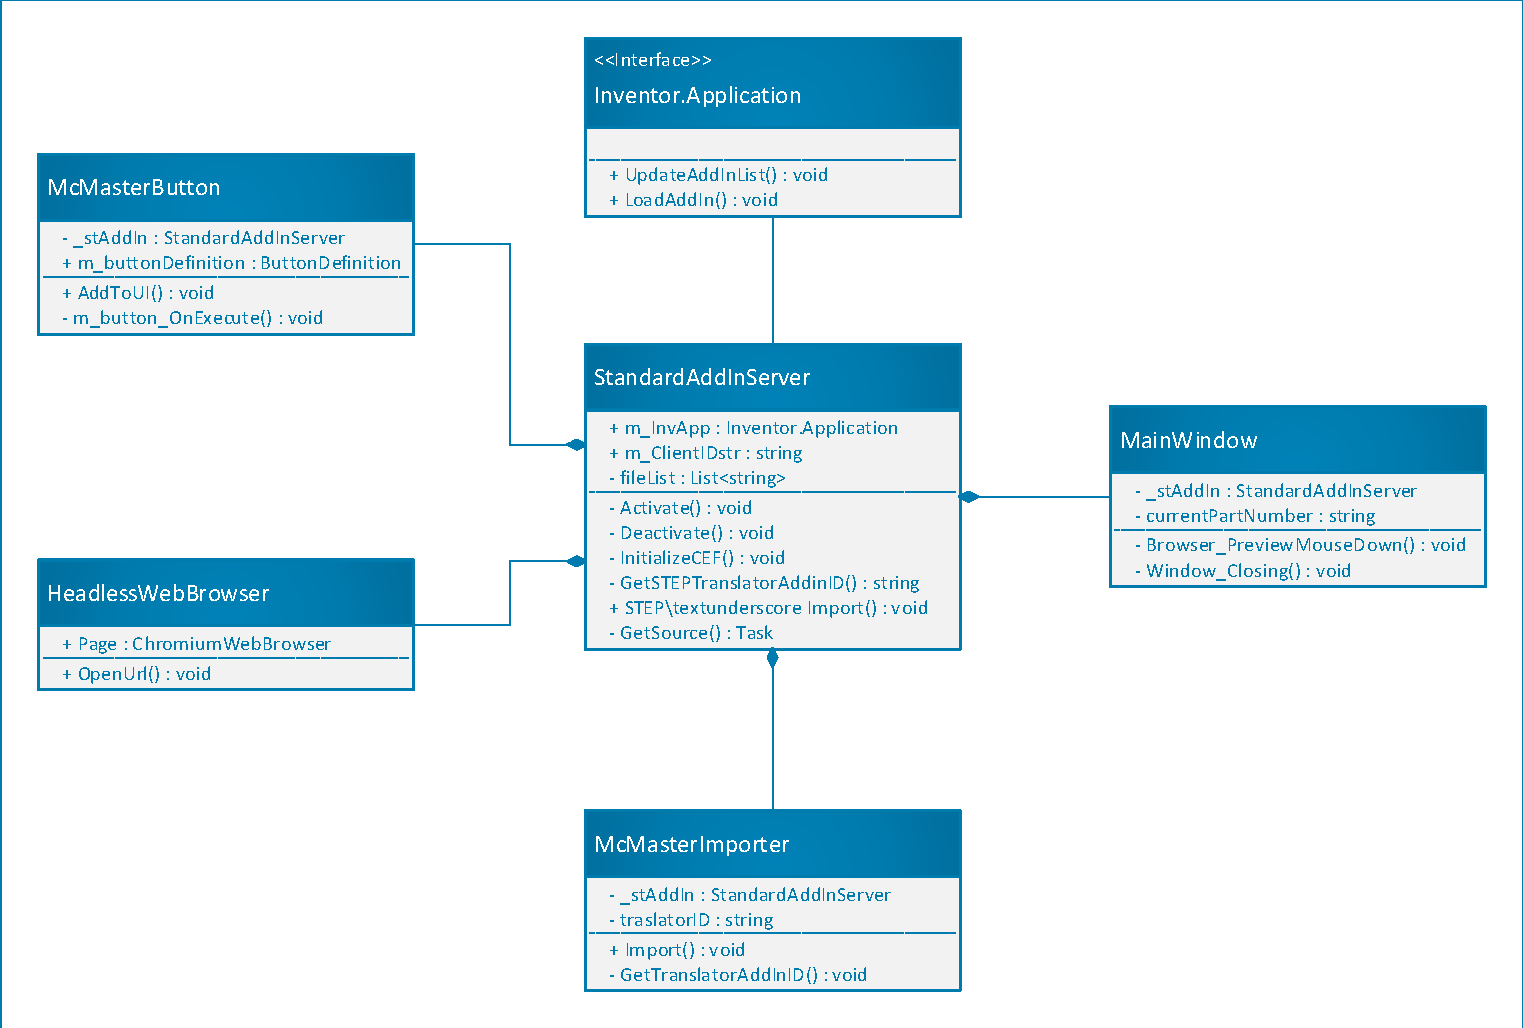
\includegraphics[width=1\textwidth]{Figures/Class_Diagram.pdf}
    \end{center}
    \caption{Use Case Diagram for User of MAFI}
\end{figure}

\subsection{Product Functionality}
MAFI will add a "button" to the ribbon interface of Inventor. Clicking this "button" will open an embedded web browser directed to www.mcmaster.com. 
From this browser the user can explore the McMaster catalog. Once the user has decided on a part they wish to retrieve a model for, the user can navigate 
to the "Add to Assembly" button that has been injected into the web browser page. This will execute a process that will convert, save, and open the selected
part's 3D model. 
\begin{figure}[H]
    \begin{center}
        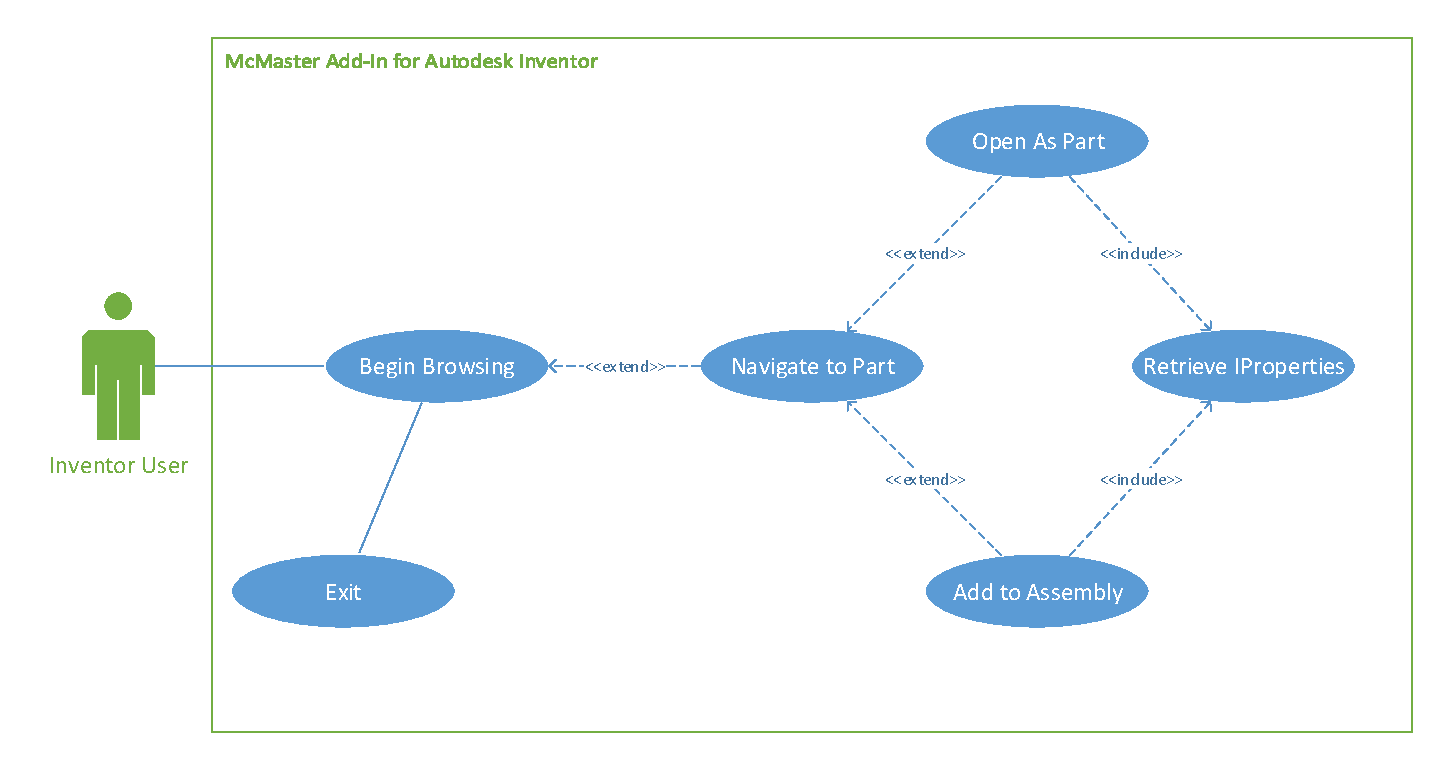
\includegraphics[width=1\textwidth]{Figures/Use_Case_Diagram.pdf}
    \end{center}
    \caption{Use Case Diagram for User of MAFI}
\end{figure}

During this process the part information data that is provided by the catalog will be added into the saved Inventor file, within it's "IProperties".
 The user is then able to continue browsing or exit the browser. The user is now able to use this file however they choose, as it has been saved to their files, and added to the project.
\subsubsection{Step by Step of Use Case}
\begin{enumerate}
    \item Begin Browsing McMaster by clicking the "Browse" button in Inventor.
    \item User chooses either to navigate to the desired part, or exits which may be done at any time from now on.
    \item If navigating to part, user chooses to either open as an individual part, to add the part directly into the assembly of various parts.
    \item Either choice will result in the retrieval of IProperties for the part.
    \item Return to step 2 until user chooses to exit.
\end{enumerate}

\subsection{Operating Environment}
MAFI will run in any Windows 64-bit environment that is capable of running the Inventor application. It is built on .NET Framework 4.7.2 Provided that Inventor has been properly installed, no additional software should be required except for the .dll library and .addin manifest provided for MAFI installation, as is outlined in the MAFI Installation Guide.
\subsection{User Interface}
\begin{figure}[H]
    \centering
    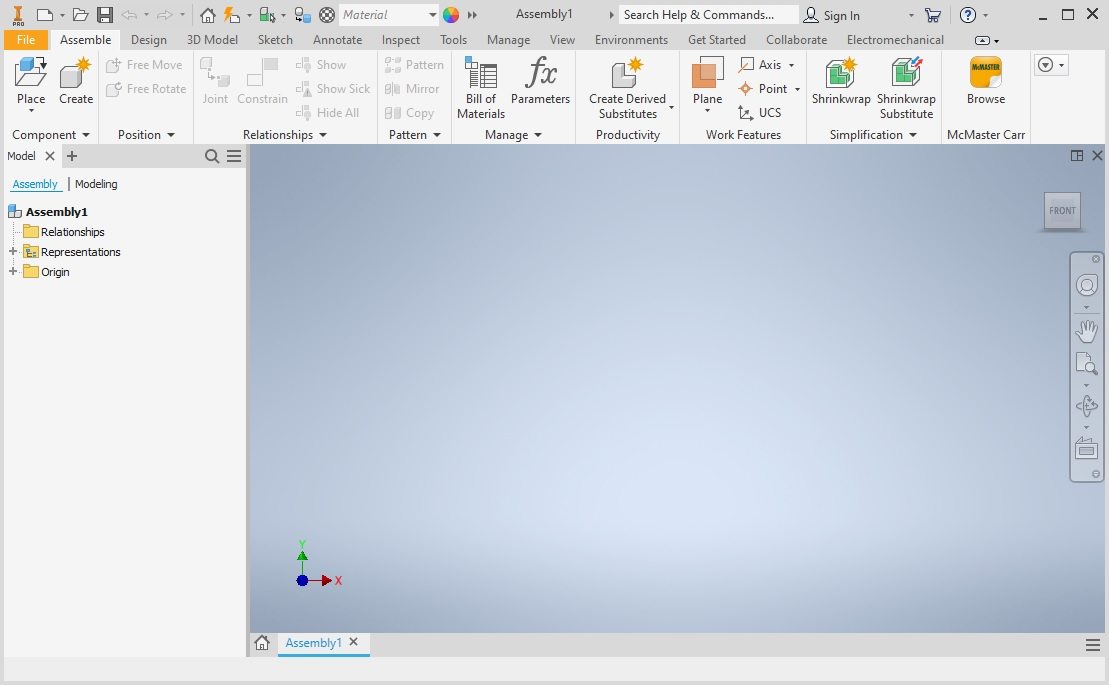
\includegraphics[width=0.5\textwidth]{Figures/mcMasterButton.JPG}
    \caption{The button(far right) addition to the ribbon interface within Autodesk Inventor.}
\end{figure}
\begin{figure}[H]
    \centering
    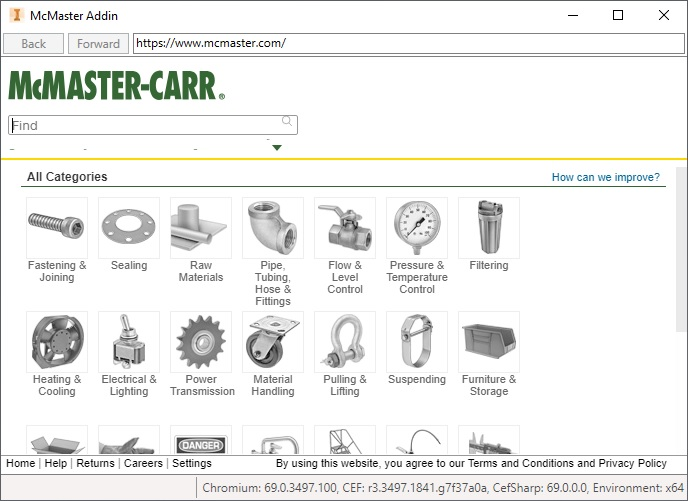
\includegraphics[width=0.5\textwidth]{Figures/webBrowserView.jpg}
    \caption{The browser instance following the button execute event.}
\end{figure}
\end{document}